%%%%%%%%%%%%%%%%%%%%%%%%%%%%%%%%%%%%%%%%%
% Jacobs Landscape Poster
% LaTeX Template
% Version 1.1 (14/06/14)
%
% Created by:
% Computational Physics and Biophysics Group, Jacobs University
% https://teamwork.jacobs-university.de:8443/confluence/display/CoPandBiG/LaTeX+Poster
%
% Further modified by:
% Nathaniel Johnston (nathaniel@njohnston.ca)
%
% This template has been downloaded from:
% http://www.LaTeXTemplates.com
%
% License:
% CC BY-NC-SA 3.0 (http://creativecommons.org/licenses/by-nc-sa/3.0/)
%
%%%%%%%%%%%%%%%%%%%%%%%%%%%%%%%%%%%%%%%%%

%----------------------------------------------------------------------------------------
%	PACKAGES AND OTHER DOCUMENT CONFIGURATIONS
%----------------------------------------------------------------------------------------

\documentclass[final]{beamer}

\usepackage[scale=1.24]{beamerposter} % Use the beamerposter package for laying out the poster

\usetheme{confposter} % Use the confposter theme supplied with this template

\setbeamercolor{block title}{fg=ngreen,bg=white} % Colors of the block titles
\setbeamercolor{block body}{fg=black,bg=white} % Colors of the body of blocks
\setbeamercolor{block alerted title}{fg=white,bg=dblue!70} % Colors of the highlighted block titles
\setbeamercolor{block alerted body}{fg=black,bg=dblue!10} % Colors of the body of highlighted blocks
% Many more colors are available for use in beamerthemeconfposter.sty

%-----------------------------------------------------------
% Define the column widths and overall poster size
% To set effective sepwid, onecolwid and twocolwid values, first choose how many columns you want and how much separation you want between columns
% In this template, the separation width chosen is 0.024 of the paper width and a 4-column layout
% onecolwid should therefore be (1-(# of columns+1)*sepwid)/# of columns e.g. (1-(4+1)*0.024)/4 = 0.22
% Set twocolwid to be (2*onecolwid)+sepwid = 0.464
% Set threecolwid to be (3*onecolwid)+2*sepwid = 0.708

\newlength{\sepwid}
\newlength{\onecolwid}
\newlength{\twocolwid}
\newlength{\threecolwid}
\setlength{\paperwidth}{48in} % A0 width: 46.8in
\setlength{\paperheight}{36in} % A0 height: 33.1in
\setlength{\sepwid}{0.024\paperwidth} % Separation width (white space) between columns
\setlength{\onecolwid}{0.30\paperwidth} % Width of one column
\setlength{\twocolwid}{0.624\paperwidth} % Width of two columns
\setlength{\threecolwid}{0.708\paperwidth} % Width of three columns
\setlength{\topmargin}{-0.5in} % Reduce the top margin size
%-----------------------------------------------------------

\usepackage{graphicx}  % Required for including images

\usepackage{booktabs} % Top and bottom rules for tables

%----------------------------------------------------------------------------------------
%	TITLE SECTION
%----------------------------------------------------------------------------------------

\title{Parallelizing Linear Recurrent Neural Nets Over Sequence Length} % Poster title

\author{Eric Martin and Chris Cundy} % Author(s)

\institute{Fill in institutes} % Institution(s)

%----------------------------------------------------------------------------------------

\begin{document}

\addtobeamertemplate{block end}{}{\vspace*{2ex}} % White space under blocks
\addtobeamertemplate{block alerted end}{}{\vspace*{2ex}} % White space under highlighted (alert) blocks

\setlength{\belowcaptionskip}{2ex} % White space under figures
\setlength\belowdisplayshortskip{2ex} % White space under equations

\begin{frame}[t] % The whole poster is enclosed in one beamer frame

\begin{columns}[t] % The whole poster consists of three major columns, the second of which is split into two columns twice - the [t] option aligns each column's content to the top

\begin{column}{\sepwid}\end{column} % Empty spacer column

\begin{column}{\onecolwid} % The first column

%----------------------------------------------------------------------------------------
%	OBJECTIVES
%----------------------------------------------------------------------------------------

\begin{alertblock}{Abstract}
RNN training and inference generally takes time linear in the sequence length because
of non-linear sequential dependencies.
We show the training and inference of RNNs with only linear
sequential dependencies can be parallelized over the sequence length using the
parallel scan algorithm, leading to rapid training on long sequences even with
small minibatch size. We use this insight and a parallel linear recurrence CUDA
kernel to accelerate several state of the art RNN architectures by up to 9x and
to solve a synthetic sequence classification task with a one million time step
dependency.
\end{alertblock}

%----------------------------------------------------------------------------------------
%	INTRODUCTION
%----------------------------------------------------------------------------------------
\begin{block}{Background}
Large minibatches are necessary for computational performance but create large memory
requirements and damage model generalization ability.

\vspace{1ex}

Linear RNNs and convolutional models such as strongly typed RNNs, Wavenet, Bytenet,
Quasi-RNNs, and simple recurrent units
have achieved state of the art results on many sequential tasks with rapid training times.

\vspace{1ex}

Given $x_t$, $\lambda_t$ can compute $h_t=\lambda_t h_{t-1} + x_t$ for $t=1\ldots T$ on $p$
processors in $O(T/p + \log(p))$ with the classic parallel scan algorithm. Backpropagation
of gradient can also be parallelized with the same algorithm.
\end{block}

\vspace{2ex}

%------------------------------------------------

\begin{figure}
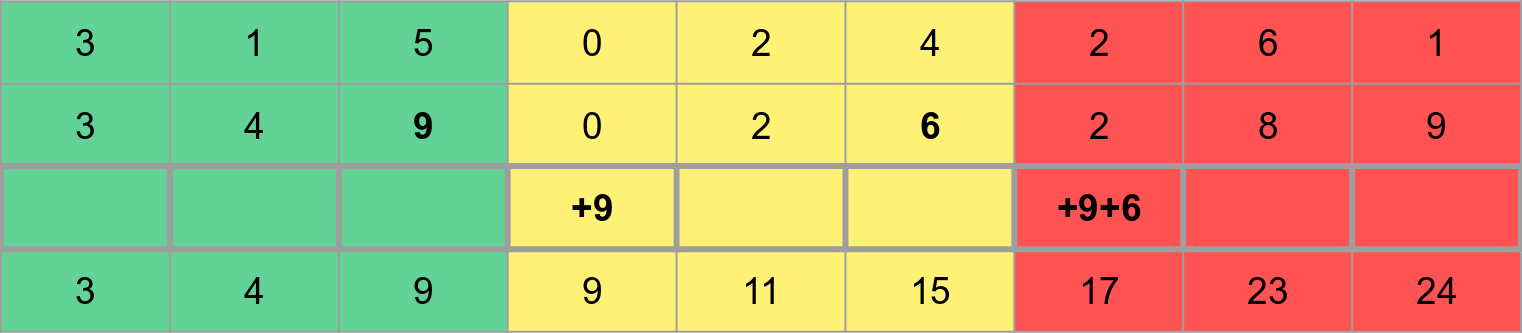
\includegraphics[width=1.0\linewidth]{cumsum.png}
\caption{Cumulative sum parallelized over 3 processors}
\end{figure}

%------------------------------------------------

\begin{block}{Gated Impulse Linear Recurrence}
Given a fast algorithm for evaluating linear recurrences, we introduce a new
linear recurrent layer called \textbf{gated impulse linear recurrence (GILR)}

\begin{align*}
g_t &= \sigma(Ux_t + b_g) \\
i_t &= \tau(Vx_t + b_z) \\
h_t &= g_t \odot h_{t-1} + (1-g_t)\odot i_t
\end{align*}
\end{block}

%----------------------------------------------------------------------------------------

\end{column} % End of the first column

\begin{column}{\sepwid}\end{column} % Empty spacer column

\begin{column}{\onecolwid} % Begin a column which is two columns wide (column 2)

%----------------------------------------------------------------------------------------
%	MATERIALS
%----------------------------------------------------------------------------------------

\begin{block}{Linear Surrogate RNNs}

RNNs have a transition function $s_t = f(s_{t-1},x_t)$. $s_t$ serves dual roles as a
summary of the past as well as the output of the unit. Non-linear $f$ in units such
as vanilla RNN and LSTM prevents parallelization over sequence length.
\vspace{1ex}

Replacing the summary of the past $s_{t-1}$ with a linear surrogate $\tilde{s}_{t-1}$
allows the easy adaption of any existing RNN architecture for parallel computation.
Several existing RNNs can be viewed as linear surrogate RNNs.
\vspace{1ex}

The state of an LSTM consists of $(c_t, h_t)$. $c_t$ is already computed
by linear recurrence, so a linear surrogate LSTM must only compute a
linear $\tilde{h}_t$. A \textbf{GILR-LSTM} uses $\tilde{h} = \text{GILR}(x)$
\end{block}

%----------------------------------------------------------------------------------------

%----------------------------------------------------------------------------------------
%	MATHEMATICAL SECTION
%----------------------------------------------------------------------------------------

\begin{block}{Accelerating Existing Linear Surrogate RNNs}
We compare the performance of several recent linear RNNs
implemented with the parallel linear recurrence kernel against
a baseline serial linear recurrence kernel.

\vspace{1ex}
\begin{table}[t]
\begin{center}
\begin{tabular}{lrrrr}
\label{table:rnn-throughput}
\small{Seq.\ Len.} & \small{SRU} & \small{QRNN(2)}
  & \small{QRNN(10)} & \small{GILR-LSTM}\\ \midrule
16 & 0.28 & 0.38 & 0.78 & 0.61\\
256 & 0.84 & 0.86 & 0.99 & 0.91\\
4,096 & 1.38 & 1.18 & 1.05 & 0.98\\
65,536 & 9.21 & 6.68 & 2.05 & 1.41\\ \bottomrule
\end{tabular}
\end{center}
\vspace{2ex}
\caption{Parallel kernel speedup for a variety of LS-RNNs.   All models use two stacked RNN layers with 256 hidden
  units, keeping the GPU memory usage constant by fixing $bT = 65,536$
  for minibatch size $b$ and sequence length $T$. QRNN($k$) refers to a
  QRNN with filter size $k$. %\citep{bradbury2017quasi}
}
\end{table}
\end{block}

%----------------------------------------------------------------------------------------
\vspace{-1ex}
\begin{figure}
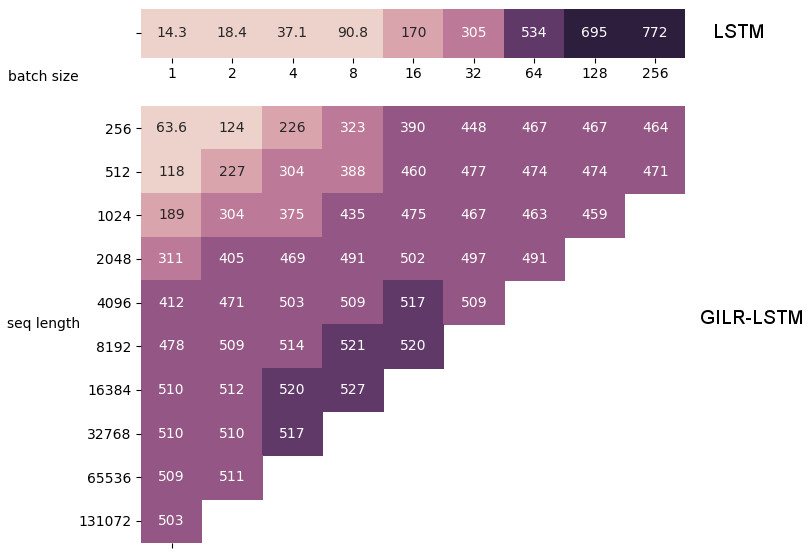
\includegraphics[width=0.9\linewidth]{cudnn_heatmap_gilr.png}
\caption{Throughput (thousand steps/s) for same sized LSTM and GILR-LSTM}
\end{figure}


\end{column} % End of column 2.1





% \begin{table}
% \vspace{2ex}
% \begin{tabular}{l l l}
% \toprule
% \textbf{Treatments} & \textbf{Response 1} & \textbf{Response 2}\\
% \midrule
% Treatment 1 & 0.0003262 & 0.562 \\
% Treatment 2 & 0.0015681 & 0.910 \\
% Treatment 3 & 0.0009271 & 0.296 \\
% \bottomrule
% \end{tabular}
% \caption{Table caption}
% \end{table}

% \end{block}

%----------------------------------------------------------------------------------------

\begin{column}{\sepwid}\end{column} % Empty spacer column

\begin{column}{\onecolwid} % The third column

\begin{block}{Synthetic Long-Term Dependency}

  We tested the GILR-LSTM by comparing to the CuDNN LSTM implementation
  on a synthetic memorisation task (problem 2b from %\citet{hochreiter1997long}. )
  We compared the performance on variants with different values of
  \(n\).  We obtained speedups of over 6x measured in wall clock time to
  convergence.  Further, the GILR-LSTM attained convergence
  when the time dependence of the problem had a length of \textbf{one  million time steps}.

 \vspace{2em}
\begin{figure}
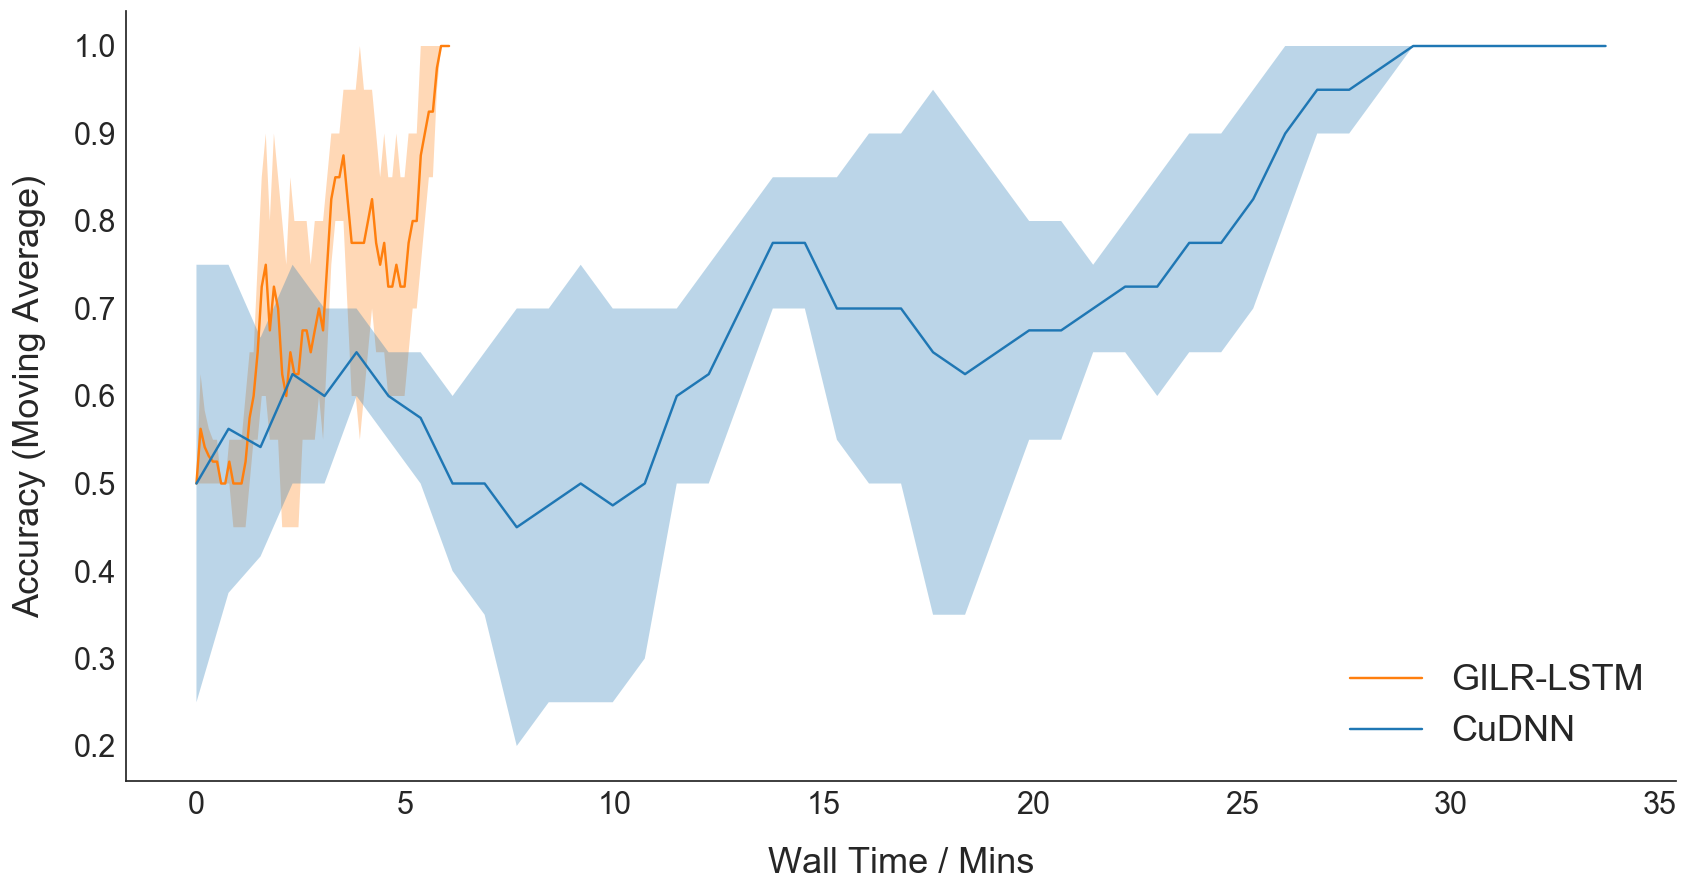
\includegraphics[width=1.0\linewidth]{8k_for_poster.png}
\caption{Accuracy on the memorisation task with 8,192 sequence length}
\end{figure}

\end{block}


%----------------------------------------------------------------------------------------
%	CONCLUSION
%----------------------------------------------------------------------------------------

\begin{block}{Conclusion}

Nunc tempus venenatis facilisis. \textbf{Curabitur suscipit} consequat eros non porttitor. Sed a massa dolor, id ornare enim. Fusce quis massa dictum tortor \textbf{tincidunt mattis}. Donec quam est, lobortis quis pretium at, laoreet scelerisque lacus. Nam quis odio enim, in molestie libero. Vivamus cursus mi at \textit{nulla elementum sollicitudin}.

\end{block}

%----------------------------------------------------------------------------------------
%	ADDITIONAL INFORMATION
%----------------------------------------------------------------------------------------

\begin{block}{Additional Information}

Maecenas ultricies feugiat velit non mattis. Fusce tempus arcu id ligula varius dictum.
\begin{itemize}
\item Curabitur pellentesque dignissim
\item Eu facilisis est tempus quis
\item Duis porta consequat lorem
\end{itemize}

\end{block}

%----------------------------------------------------------------------------------------
%	REFERENCES
%----------------------------------------------------------------------------------------

\begin{block}{References}

\nocite{*} % Insert publications even if they are not cited in the poster
\small{\bibliographystyle{unsrt}
\bibliography{sample}\vspace{0.75in}}

\end{block}

%----------------------------------------------------------------------------------------
%	ACKNOWLEDGEMENTS
%----------------------------------------------------------------------------------------

\setbeamercolor{block title}{fg=red,bg=white} % Change the block title color

\begin{block}{Acknowledgements}

\small{\rmfamily{Nam mollis tristique neque eu luctus. Suspendisse rutrum congue nisi sed convallis. Aenean id neque dolor. Pellentesque habitant morbi tristique senectus et netus et malesuada fames ac turpis egestas.}} \\

\end{block}

%----------------------------------------------------------------------------------------
%	CONTACT INFORMATION
%----------------------------------------------------------------------------------------

\setbeamercolor{block alerted title}{fg=black,bg=norange} % Change the alert block title colors
\setbeamercolor{block alerted body}{fg=black,bg=white} % Change the alert block body colors

\begin{alertblock}{Contact Information}

\begin{itemize}
\item Web: \href{http://www.university.edu/smithlab}{http://www.university.edu/smithlab}
\item Email: \href{mailto:john@smith.com}{john@smith.com}
\item Phone: +1 (000) 111 1111
\end{itemize}

\end{alertblock}

\begin{center}
\begin{tabular}{ccc}

\includegraphics[width=0.4\linewidth]{logo.png} & \hfill & 
\includegraphics[width=0.4\linewidth]{logo.png}
\end{tabular}
\end{center}

%----------------------------------------------------------------------------------------

\end{column} % End of the third column

\end{columns} % End of all the columns in the poster

\end{frame} % End of the enclosing frame

\end{document}
